\section{Introduction}

\begin{definition}[\textit{Task}]
    In the context of OS, a task is defined as a basic unit of work or a program that is scheduled for execution. 
    It represents an instance of a program in execution, including its code, data, and context.
\end{definition}
In Linux, a task is the common factor between a Unix process and a thread. 
Threads are tasks that shares the same address space, while a process is a single task. 

\subsection{Task control block}
Each task in linux is represented into the memory with a structure called \texttt{task\_struct}. 
The OS manages a list of \texttt{task\_struct} to manage all the tasks and also an hash table to simplify certain operations. 

For some hardware we need to add the \texttt{thread\_info} structure at the end of the kernel mode stack to reach the \texttt{task\_struct}.
This is helpful when the number of registers is limited. 

The main elements of \texttt{task\_struct} and \texttt{thread\_info} are: 
\begin{itemize}
    \item \texttt{thread\_struct}: used for selecting the correct tasks when performing a context switch. 
    \item \texttt{preempt\_count}: avoid context swith if the current process is interacting directly with the kernel. 
        The context swith is negated when this integer (in the active task) is greater than zero. 
    \item \texttt{mm\_struct}: this structure describes the memory layout of the task (only the process accessible space). 
    \item \texttt{task\_struct}: describes the task state. 
\end{itemize}
The most important task states are shown in the following diagram. 
\begin{figure}[H]
    \centering
    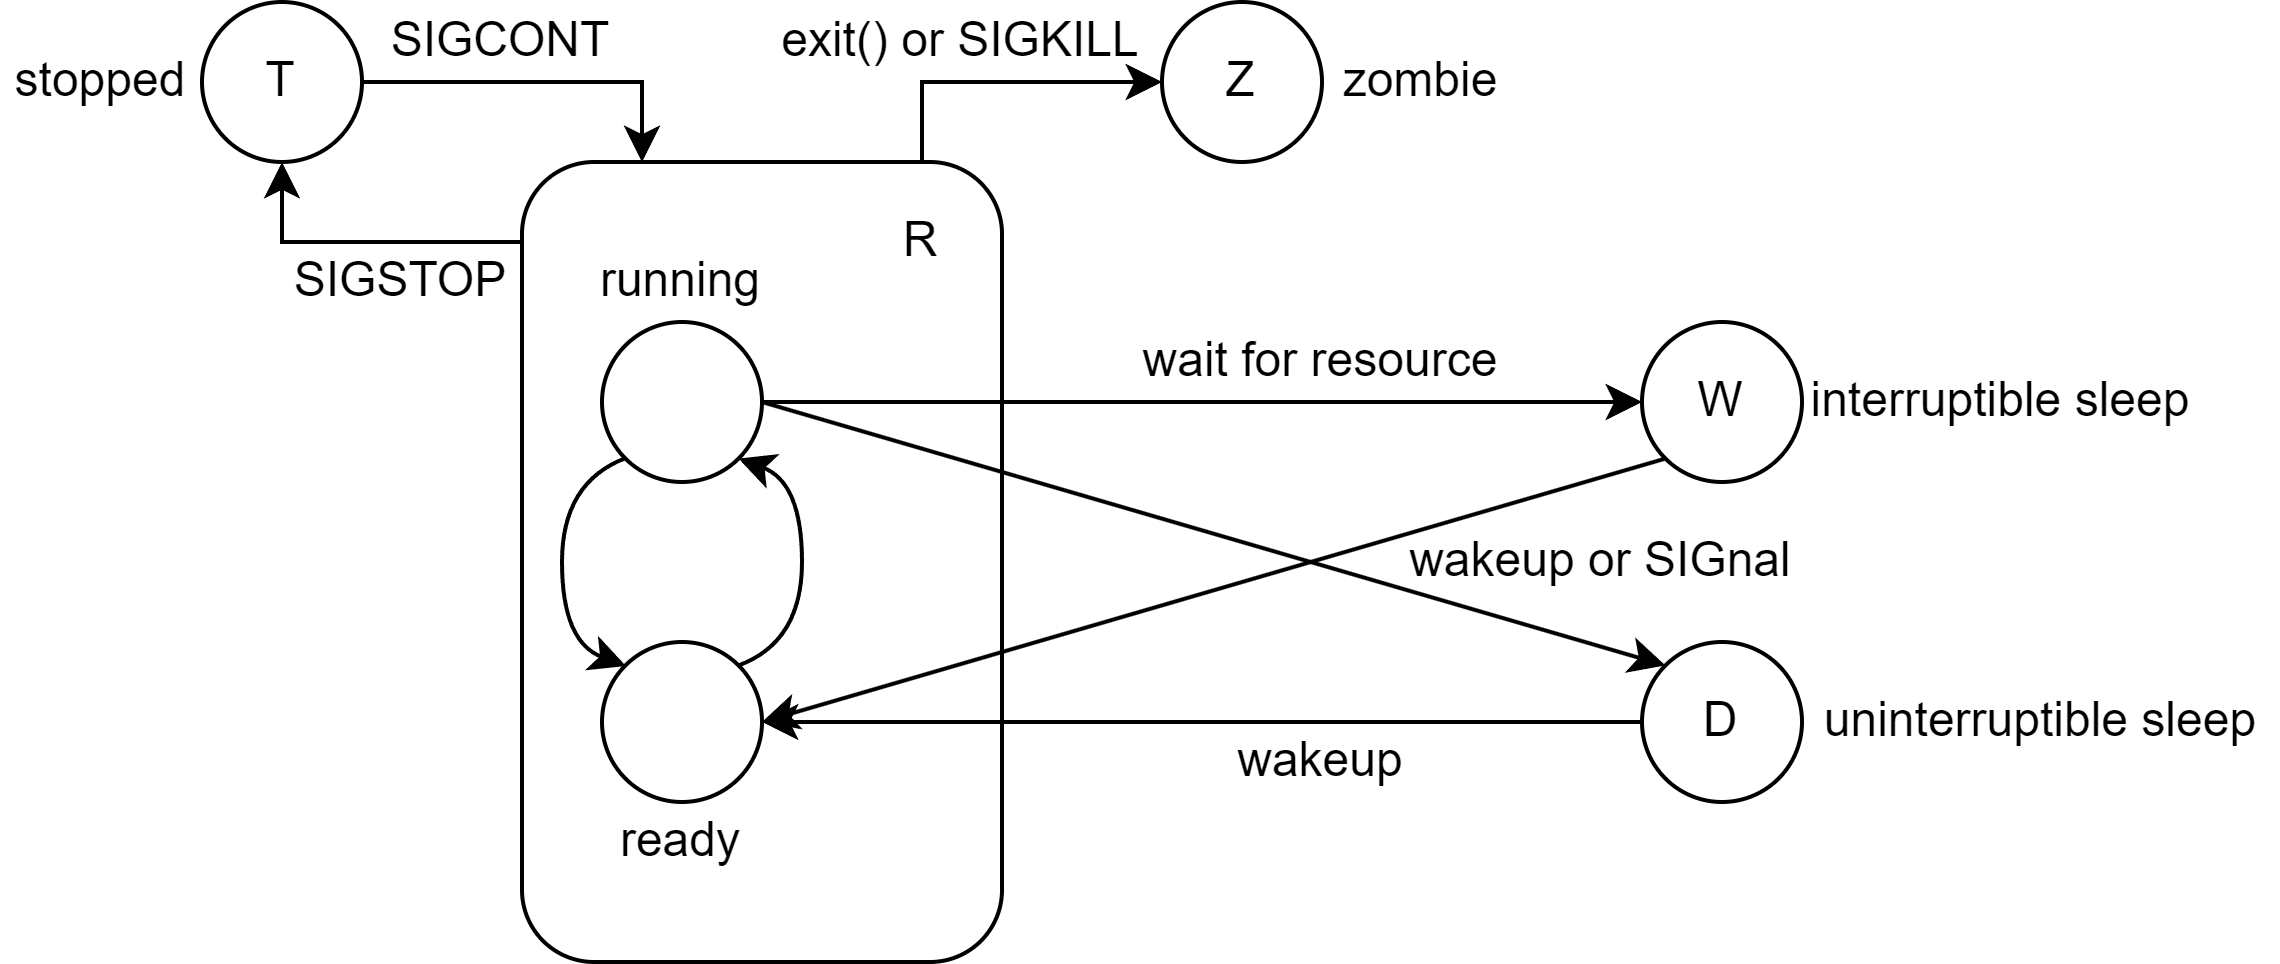
\includegraphics[width=0.75\linewidth]{images/proc.png}
    \caption{Tasks states}
\end{figure}
In kernel code, you typically enter the wait state and queue with \texttt{wait\_event} and \texttt{wait\_event\_interruptible} calls, respectively.
The queue is used to schedule the tasks execution. 